\documentclass{report}

\usepackage[T1]{fontenc}
\usepackage[utf8]{inputenc} % also latin5
\usepackage[turkish,shorthands=:!]{babel}
\usepackage{indentfirst}

%% Sets page size and margins
\usepackage[top=3cm,bottom=2cm,left=3cm,right=3cm,marginparwidth=1.75cm]{geometry}

%% Useful packages
\usepackage[colorlinks=true, allcolors=blue]{hyperref}
\usepackage{graphicx}

% Specify bibliography package
\usepackage{natbib}
% ----------------------------------------------------------------------

\title{Théodore Géricault'nun Medusa'nın Salı Tablosunun Müzikteki Doku Kavramı Üzerinden İncelenmesi}
\author{Şahin Kureta - 22083802}
\date{Müzisyenler için Terminoloji II: 2023 Güz Final Ödevi}
% ----------------------------------------------------------------------

\begin{document}
\maketitle

\section*{Giriş}
Théodore Géricault 26 Eylül 1791 tarihinde Fransa'nın Rouen şehrinde doğmuş, 26 Ocak 1824'te Paris'te ölmüştür.
Babası Georges-Nicolas Géricault varlıklı bir avukat ve işadamıdır.
1806 yılında klasik eğitimi ile ünlü Lycée Impérial'de öğrenimine başlamış ve 1797 Grand Prix de Rome ödülünü alan Fransız ressam Pierre Boullion ile çalışmıştır.
Daha sonra Carle Vernet ve Pierre-Narcisse Guérin ile çalışmaya devam etmiştir.
Öğrenimine École des Beaux Arts'da devam etmiştir \citep{kronzek2023}.

\begin{figure}[htp]
    \centering
    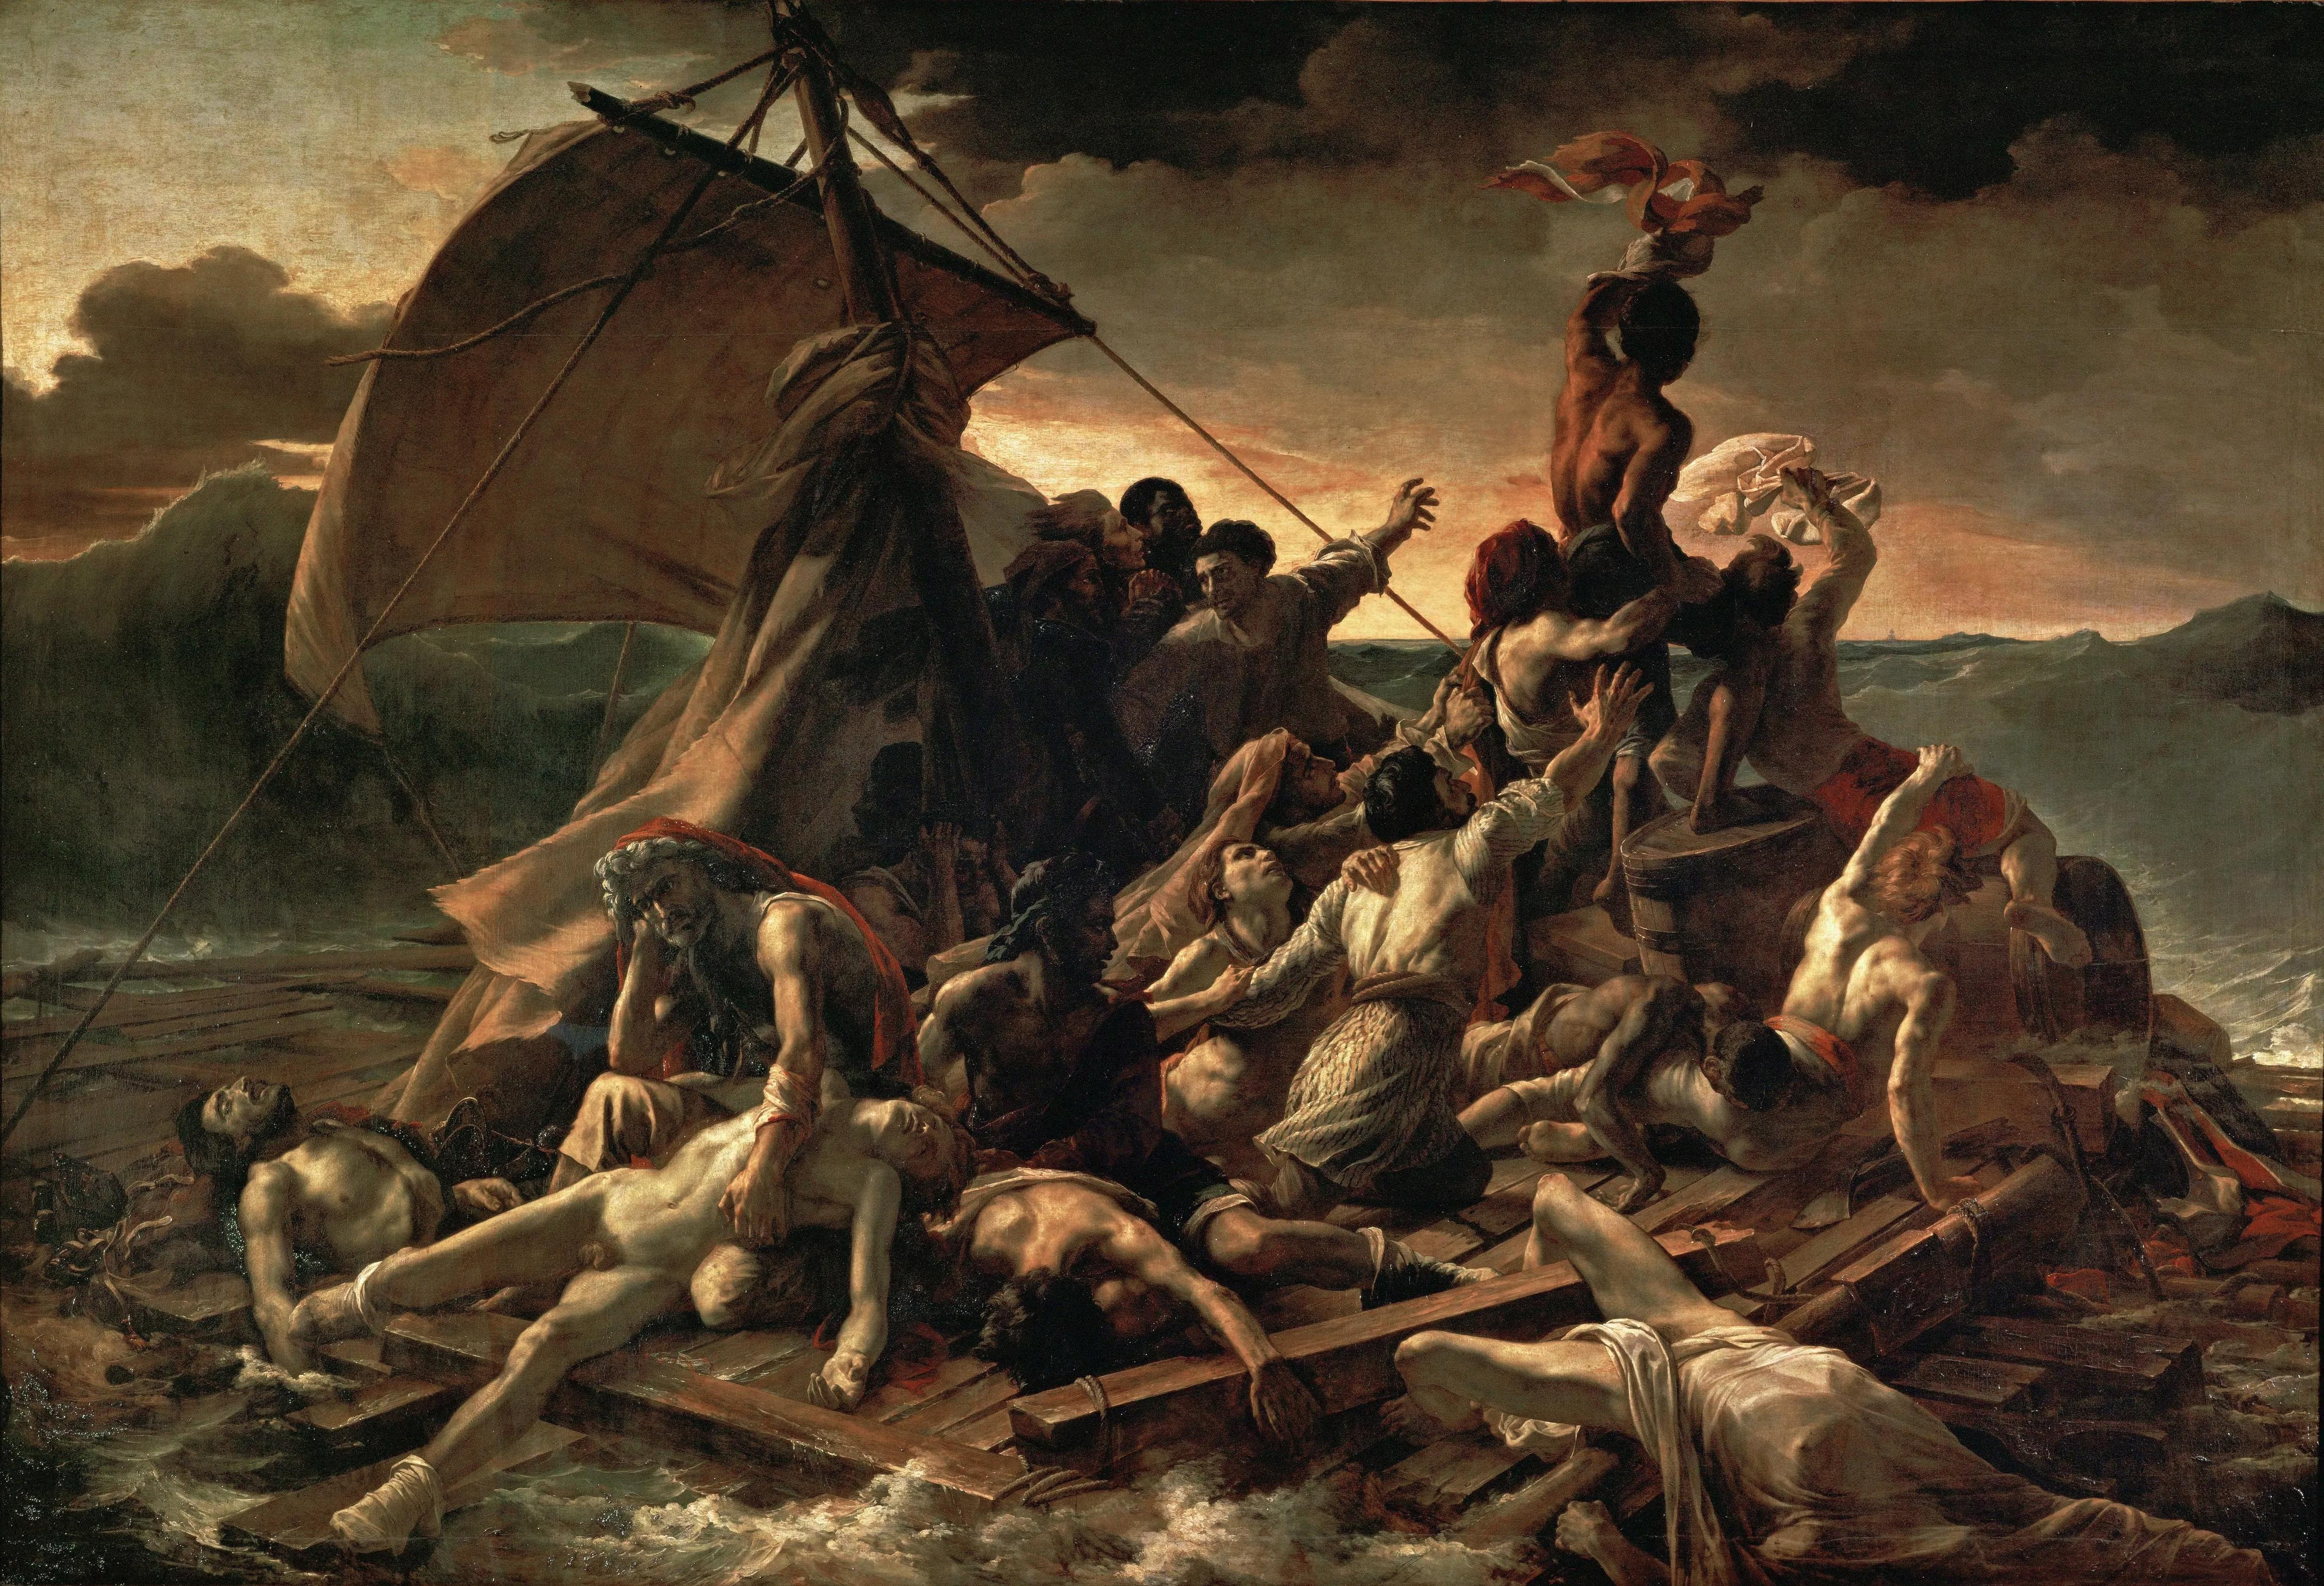
\includegraphics[width=14cm]{medusa}
    \caption{Medusa'nın Salı}
    \label{fig:medusa}
\end{figure}

1818-1819 yılları arasında on sekiz ay boyunca hayatının en önemli eseri olan \textit{Medusa'nın Salı (Le Radeau de la Méduse)} üzerinde çalışmış ve 27 yaşındayken eseri tamamlamıştır.
Bu resim o dönemde meydana gelen tartışmalı bir olayı konu almıştır.
Medusa isimli bir devlet fırkateyni, siyasi himaye ve adam kayırma sayesinde işe alınmış bir kaptanın beceriksizliği yüzünden Afrika kıyılarında batmıştı.
Hatalı kaptan ayrıca en sağlam filikaları kendisi ve arkadaşları için almış ve geri kalan yolcuları batan geminin parçalarından derme çatma bir sal yapmak zorunda bırakmıştı.
Bu salda mahsur kalan 149 kişiden yalnızca on beşi hayatta kalabilmiş ve salda yamyamlık gibi dehşet verici olaylar yaşanmıştı \citep{kronzek2023}.

\section*{Ressamın Hazırlıkları ve Çalışma şekli}
1816 tarihli gemi kazasından çok etkilenen Géricault 1818 yılının başlarında kazadan kurtulan iki kişiyle görüşmeler yapmaya başlamıştır: cerrah Henri Savigny ve École nationale supérieure d'arts et métiers'de mühendis Alexandre Corréard.
Resmin genel havasını en çok bu iki kişinin duygusal tasvirleri belirlemiştir \citep{riding2003}.
Géricault önceki seyahatlerinde akıl hastalığının ve vebanın mağdurlarını gözlemlemişti ve Medusa için araştırma yaparken gerçekçi olma çabaları nedeniyle cesetlerin katılığını bir saplantı haline getirmişti.
Ölü vücutların renk tonlarını en doğru şekilde tasvir edebilmek için Beaujon hastanesinin morgundaki kadavraların eskizlerini çizmiş, ölmek üzere olan hastaların yüzlerini etüd etmiş, çürümelerini incelmek için stüdyosuna kopmuş uzuvlar götürmüş ve bir akıl hastanesinden ödünç aldığı kesilmiş kafayı stüdyosuna götürüp 2 hafta boyunca onu çizmiştir \citep{trapp1976}.

\section*{Eserin Dokusu}
Medusa'nın Salı 491 cm x 716 cm boyutlarında, oldukça büyük bir resimdir \citep{louvre2024}.
Derme çatma salın üstündeki umutsuz ve çaresiz insanların ufukta bir gemi görüp kurtulduklarını anladıkları anı resmetmektedir.
Gemi bu dev tabloda bile küçücük kalmıştır.
Resmin Kompozisyonu salın yelken direği ve halatlarının ve ufuktaki gemiye işaret eden insanların oluşturduğu, üst üste gelen iki piramit şeklindedir.
Ancak bu resme müzikal bir gözle baktığımızda dikkatimizi çeken bir başka şekil daha vardır: resimdeki insan figürleri soldan sağa bir \textit{crescendo} işareti gibi yükselmektedir.
Bakışımızı bu soldan sağa harekete odakladığımızda bir şey daha dikkatimizi çeker: resim en soldan yalnızca gövdesi kalmış bir ceset, çaresizlikten belki şok halinde donakalmış bir adam, umutla uzanan eller, bayrak sallayan insanlar ve en sağda ufuktaki gemi ile \textit{macabre}, ölüm ve çaresizlikten umut ve kurtuluşa gitmektedir.
Denizin durumu bile bu kötüden iyiye gidişle paralel olarak değişir, sakinleşir.
Bu gidişin sonundaki minicik gemi bize minör tondaki karanlık ve umutsuz dev bir eserin sonunda, yalnızca bir notanın (tonun üçüncü derecesinin) yarım ses tizleştirilmesiyle (Picardi üçlüsü) bitmesiyle birden parlayan umut hissini çağrıştırır.

Eserdeki bu soldan sağa net hareket ve üst üste resmedilen insan figürleri göz önünde buludurulduğunda resmin en yakın olduğu müzikal dokunun polifonik doku olduğu söylenebilir.
Resmin alt yarısında ölüm ve umutsuzluktan oluşan, üst yarısında da çaba ve umudu temsil eden bir hattın olduğu da görülmektedir.
Hatta muhtemelen bu inanılmaz ızdırabın sürekli arka planını teşkil etmiş olan, denizi bir \textit{ostinato} (İtalyanca inatçı; sürekli tekrar eden motif ya da cümle) olarak değerlendirirsek bu eseri bir \textit{passacaglia}'ya (genellikle üç zamanlı bir bass ostinato üzerine yazılmış ciddi karakterli eser) benzetmek de mümkündür.
Resim doğası itibariyle durağan, tek bir anın temsil edildiği bir medyum olsa da, ressam bu eserde denizde kaybolan insanların çaresizliklerinin zirvesinden, kurtuldukları ana kadar geçen zamanı ustalıkla tasvir etmiştir.
İzleyici olarak biz de bu yolculuğun insanların bu derme çatma salı ilk bir araya getirip üzerine yerleştikleri ve görece umut ve yaşama arzusu dolu oldukları anından başlayarak, durumlarının giderek kötüleştiği, karanlıklaştığı ve bir anlamda \textit{disonant} hale geldiği anına kadarki kısmını hayal edersek, arka planda varlığını asla unutturmayan deniz ostinatosu ile birlikte sadelikten karmaşıklığa ilerleyen passacaglia formu ile kurulan benzerliğin hiç de zorlama olmadığı söylenebilir.
Eser Fransız Romantizmi'nin simgelerinden biri haline gelmiş olsa da Caravaggio benzeri bir stilde \textit{chiaroscuro} (İtalyanca aydınlık-karanlık; kompozisyonun genelinde yüksek kontrast kullanımı) ve \textit{tenebrism} (İtalyanca tenebroso kelimesinden; karanlık, kasvetli, gizemli) kullanımı esere son derece Barok bir hava vermektedir.
Barok dönemde polifoni sanatının zirve yaptığı ve passacaglia formunun en önemli eserlerinin de bu dönemde yazıldığı göz önüne alındığında resmin polifonik doku ve passacaglia formu ile olan ilişkisi bir kez daha desteklenmektedir.

\bibliographystyle{apalike}
\bibliography{references}

\end{document}
